\documentclass[a4paper]{article}
\usepackage{amsmath}
\usepackage{amssymb}
\usepackage{graphicx}


%%%%lualatex on
%\usepackage{luatextra}
%Ligatures={Contextual, Common, Historical, Rare, Discretionary}
%\setmainfont[Mapping=tex-text]{Linux Libertine O}

\usepackage{natbib}

\title{Note about WSC}
\author{Simon}
\begin{document}
\maketitle
\section{Classic Cultural Evolution}





The cultural evolution's literature gives us a way to interpret evolution of cultural artifact such as those produce in economical field. We want to confront well know cultural evolution's mechanism to well known economical evolution's mechanism and see and show their differences.

\subsection{Statistical Analysis}
In order to test if the data fit power law curve aand to know the parameters off such learning curve, we will used to R Cran Package poweRlaw \cite{gillespie2015fittingheavytaileddistributionsthepowerlawpackage} wich is based on \cite{clauset2009powerlawdistributionsinempiricaldat}. This package allow us to fit the datas with a power law and to know the parameters of this fitted power law ($\alpha$). Moreover, it allows use to test if the datas are actually following the fitted power law using a bootstrapping method that calcul kolmogorv smirnov coefficient.

\subsection{Verification}

First we verify that our model implements well the already known cultural evolution mechanisms.

Here we follow \cite{mesoudi2009randomcopyingfrequencydependencopyingandulturechange,bentley2004randomdriftandculturechange} and look for the evolution of a single traits depending on the innovation rate $\mu$ in a 250 agents population during 1000 steps.


With infinite innovation possibilities(ie : $n$ variant $| n\in\mathbb{A} $) the results, showed in the figure \ref{fig:allMutation} are the same that those from \cite{bentley2004randomdriftandculturechange}.
\begin{figure}[hbp]
	\begin{center}
		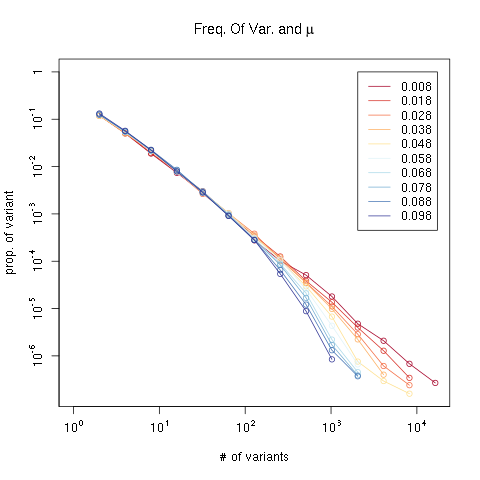
\includegraphics[width=7cm]{img/allmuRandMax.png}
	\end{center}
	\caption{rand()\%RAND\_MAX}
	\label{fig:allMutation}
\end{figure}


And as them we find the same between $\alpha$ and $\mu$ (cf tab :\ref{tab:mualpha} \& tab \ref{tab:Bmualpha}).
\begin{figure}[hbp]
	\begin{center}
		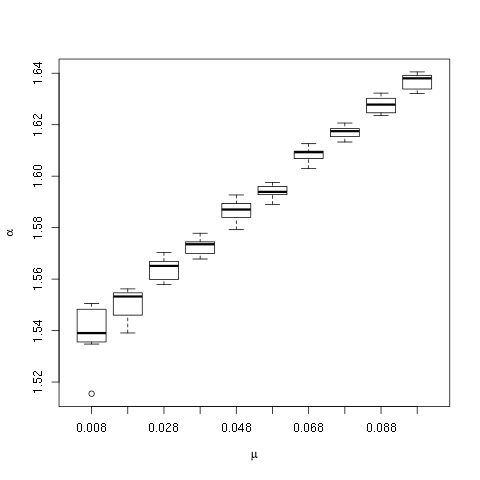
\includegraphics[width=7cm]{img/alphawrtmu.png}
	\end{center}
	\caption{$\alpha$  wrt. $\mu$ }
	\label{fig:alphamu}
\end{figure}

\begin{table}
	\centering
	\begin{tabular}{l|cc}
			$\mu$ & $\alpha$ & SD\\\hline
			0.008&1.539122&0.010154623\\
			0.018&1.550888&0.005487468\\
			0.028&1.564014&0.004155942\\
			0.038&1.572597&0.003297191\\
			0.048&1.586550&0.003965373\\
			0.058&1.593909&0.002497322\\
			0.068&1.608492&0.003090030\\
			0.078&1.617235&0.002188951\\
			0.088&1.627801&0.003247013\\
			0.098&1.637116&0.002900783\\
	\end{tabular}
	\caption{Mean \& SD are done with 10 run for each $\mu$}
	\label{tab:mualpha}
\end{table}







\begin{table}
	\centering
	\begin{tabular}{l|cc}
$\mu$&$\alpha$&(SD)\\\hline
0.004&1.50&(0.02) \\
0.008&1.52&(0.02)\\
0.016&1.55&(0.03)\\
0.032&1.59&(0.06)\\
0.064&1.78&(0.08)\\
0.128&1.99&(0.04)\\
	\end{tabular}
	\caption{Mean \& SD from \cite{bentley2004randomdriftandculturechange} }
	\label{tab:Bmualpha}
\end{table}







\subsection{generalisation: Multiple Traits (all varying on $\mathbb{N}$)}
Once the results are verified, we generalized those result for $n$ possible traits.

In that case individual owns a vector of $n$ traits (price in our experiment). When a cultural exchange occurs the whole vector is exchanged and each traits  had a $\mu$ probability to mutate.

Here we check that it does not change the result of the algorithm in the long terms and that each traits will evolve following the same curves than when just one trait is evolving. The results are shown in figures \ref{fig:10resources}. Those results are statistically the same than those from the previous experiments.

\begin{figure}[h]
	\begin{center}
		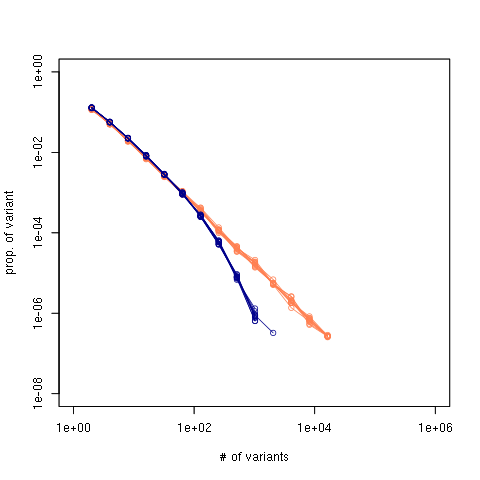
\includegraphics[width=6cm]{img/10resources.png}
	\end{center}
	\caption{$\mu=\{.08,.098\}$ for 10 resources}
	\label{fig:10resources}
\end{figure}




\section{Cultural Mechanisms Comparison with economical evolution}

Now that we have shown that our model reproduce well the well known cultural evolution mechanisms, and that even when multiple price are simultaneously evolved, we will compare the evolution of the system when it is submit to different mechanisms of transmission and innovation. The one we will use and compare with those used previously are those used by \cite{gintis2006theemergenceofapricesystemfromdecentralizedbilateralexchange}.

\subsection{Framework Adjustment}
In order to allow such comparison we will do our simulation using the same parameters used by Gintis which are : a population with 100 agents per good assuming six good so 600 agents evolving during 1500 steps and with a innovation rate of .01.

It worth to notice here than the way Gintis counts the steps is slightly different than the others article. Indeed in Gintis agents follow 10 Produce/Trade/Consume cycles before exchanging their cultural belief, which means than when in the previous runs we speak about 5 runs, it means in Gintis framework ``5 cycle of cultural exchange'' so 50 steps.

The results are those expected : given the much higher number of agents and 


\subsection{Gintis' imitation mechanism}
The imitation mechanism is ``score biased'', meaning that people tends to copy the price vector of other that exhibits a high score. This score is computed using the utility function and is summed for every 10 step during a evaluation periode. After those 10 step of evaluation the exchange is done between agents  

In its new paper agents adapt themselves using learning simple rules that could be useful to have quicker improvement (and a more cognitively accurate model):

\begin{quotation}
	After each trading period, agents consume their consumption inventories provided they have a positive amount of each consumption good, and agents replenish their inventories of their production goods. Moreover, each trader updates his private price vector on the basis of his trading experience over the period, raising the price of a consumption or production good by 0.02\% if his inventory is empty (i.e.,if he failed to purchase any of the consumption good or sell all of his production good), and lowering price by 0.02\% otherwise (i.e., if he succeeded in obtaining his consumption good or sold all his production inventory).In general, it would be desirable to allow this adjustment strategy to evolve endogenously according to learning or imitation processes, but I have not investigated this possibility.
	\\\cite[p. 7]{gintis2010thedynamicsofgeneralizedmarketexchange}
\end{quotation}

\subsubsection{The utility function \& Barter Process}
The utility function is computed depending on the quantity that agent had collected during the trade. Those quantities are themselves defined by the Barter Process in order to maximise this utility function and depend on the private price of both trader.

\subsection{Gintis' innovation mechanism}




\subsection{Comparison}
In order to compare the different mechanisms used in the different paper we will cross them  following the table \ref{tab:exp}.
\begin{table}
	\centering
	\begin{tabular}{l|c|c}
		& Rand & Gintis \\\hline
		$\mu$ &A & B \\
		$\mu +\alpha$ & C & D \\
	\end{tabular}
	\caption{Experimental Setup}
	\label{tab:exp}
\end{table}


First we check how those different mechanisms impact the power law distribution.

\begin{figure}[hbp]
	\begin{center}
%		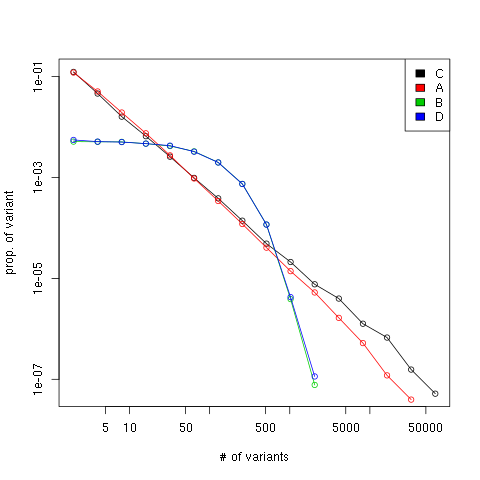
\includegraphics[width=6cm]{img/powerABCD.png}
	\end{center}
	\caption{power law for each exp define in table \ref{tab:exp} after 2000 step}
	\label{fig:powerABCD}
\end{figure}

As expected depending on the selection process the repartition follow a power law (random selection) or a exponential law).

Next let's have a look which combination lead to the right economical processes.

\begin{table}
	\centering
	\begin{tabular}{l c c}
		& Random Transmission & Gintis Transmission \\
		FRI & \raisebox{-.5\height}{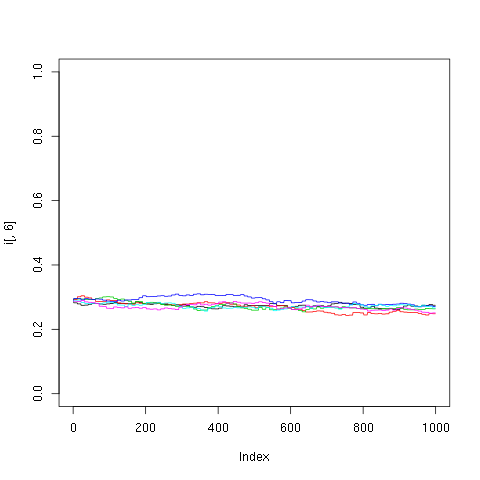
\includegraphics[width=5cm]{img/sdEvolEXP2.png}}&\raisebox{-.5\height}{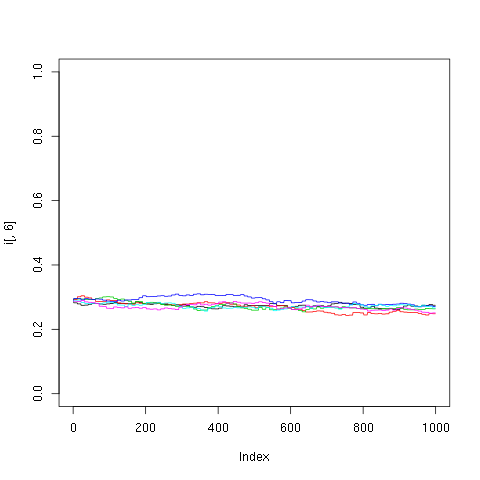
\includegraphics[width=5cm]{img/sdEvolEXP2.png}} \\
		GRI & \raisebox{-.5\height}{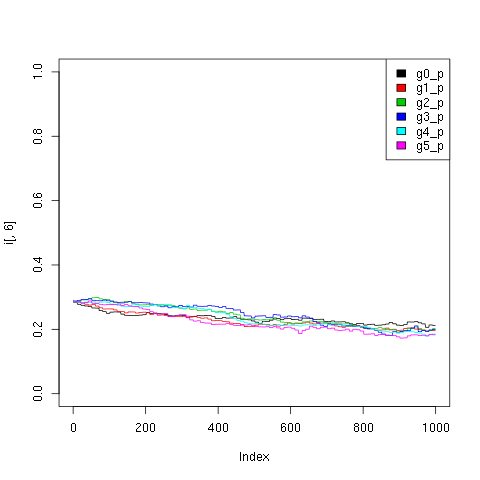
\includegraphics[width=5cm]{img/sdEvolEXP3.png}}&\raisebox{-.5\height}{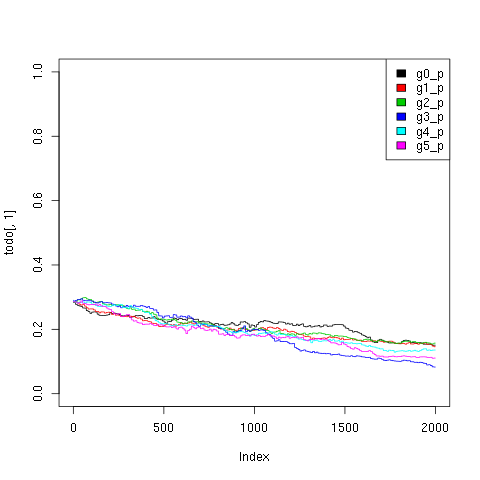
\includegraphics[width=5cm]{img/sdEvolEXP4.png}}

	\end{tabular}
	\caption{Evolution of SD. FRI : Fully Random Innovation, GRI: Gintis Random Innovation}
	\label{tab:sdevol}
\end{table}

\section{Other reflexion}
\subsection{Discrete and finite inovation space}
The Finite Innovation Effect (ie : $n$ variant  $| n\in\{0,\cdots,100\}$). If choose a innovation mechanism such as the number of possible new variant is finite, we see a strange ``anticonformist-like'' effect such the one shown by \cite{mesoudi2009randomcopyingfrequencydependencopyingandulturechange}. This effect is visible in the figure \ref{fig:finitEffect}.
\begin{figure}[h]
	\begin{center}
		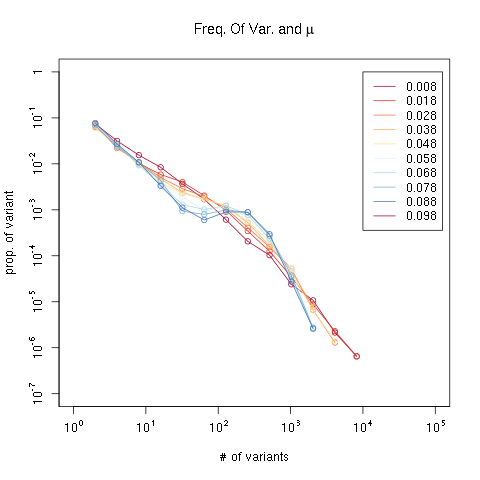
\includegraphics[width=7cm]{img/allmu.png}
	\end{center}
	\caption{rand()\%100}
	\label{fig:finitEffect}
\end{figure}

\subsection{Validation of the curves similarities}
\begin{figure}[h]
	\begin{center}
		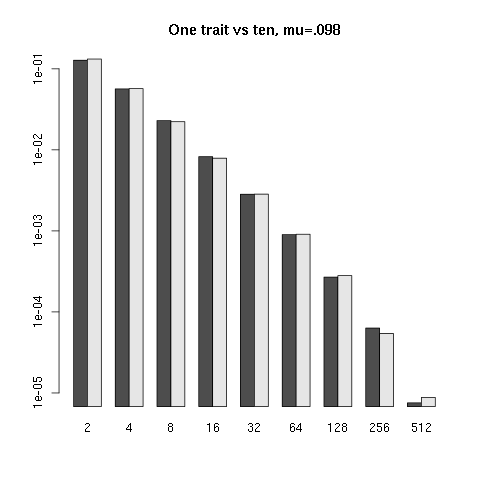
\includegraphics[width=6cm]{img/OneVsTenMu098.png}
		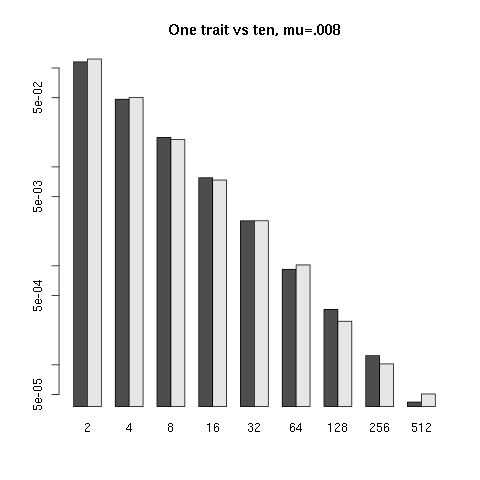
\includegraphics[width=6cm]{img/OneVsTenMu008.png}
	\end{center}
	\caption{$\mu=\{.08,.098\}$ for one of the 10 resources VS one only}
	\label{fig:OneVsTen}
\end{figure}
\bibliographystyle{apalike}
\bibliography{/home/scarrign/Documents/biblio/bib/phd.bib}  
\end{document}


